%!TEX root = ../Report.tex

\section{Interesting Use Cases - Reasoning}

In order to be able to do our investigations, we need to select a coupele of interesting use cases of stencil code.

The potential for experiments is massive, due to the large amount of variables we have access to. In our investigation, we have access to the following:

EXPAND UPON THESE

\begin{enumerate}
	\item Number of iterations
	\item Thread pinning
	\item Combinations of multiple different workloads
	\item Grid size
	\item Number of workers
\end{enumerate}

All of these can be changed from stage to stage. Beyond these parameters, we can have many different combinations of programs running simultainiously. 

For the purposes of this project, we will select a few interesting use cases of the stencil pattern, and focus on testing these in a few different configurations.



\section{Finding Interesting Use Cases}

In order to find interesting use cases, we performed an inital foray into the experiment space we have access to.

\subsection{First}

Firstly we compared the performance characteristics of each of our different workloads, and how they performed with different numbers of threads.

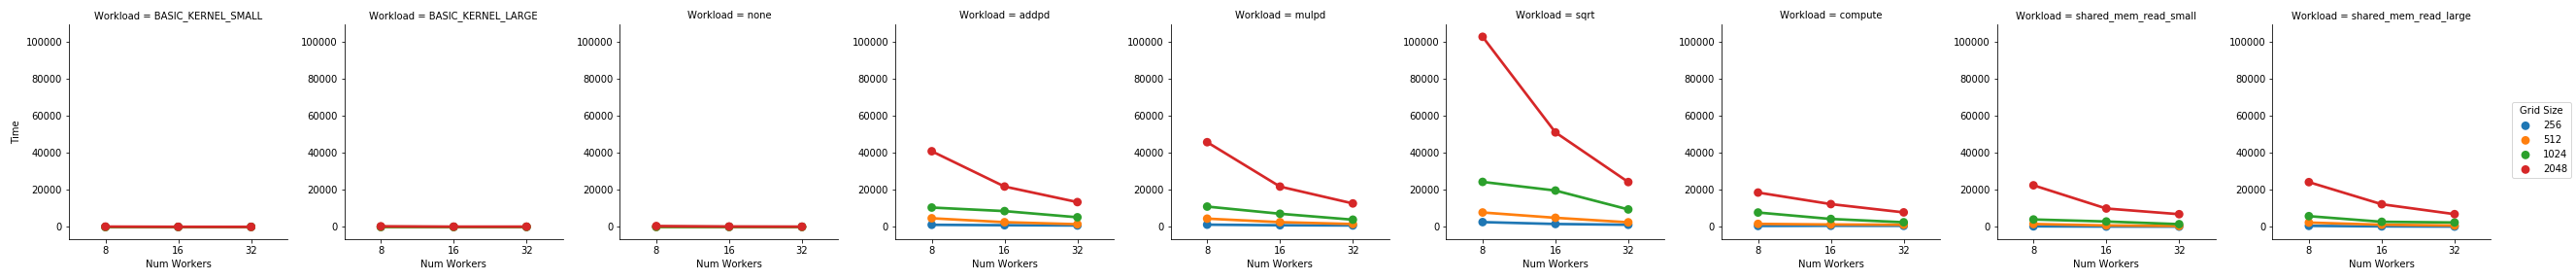
\includegraphics[width=1\textwidth]{graphics/quicktest.png}

\subsection{Second}

Next we picked some interesting kernels form the previous experiment, and investigated them further, with some smaller grid sizes. This was because we were interested in a use case where at a certain point, adding more threads is no longer optimal.

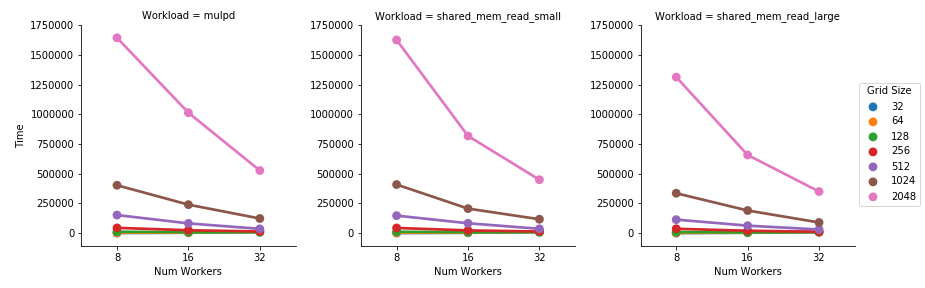
\includegraphics[width=1\textwidth]{graphics/focustest2_1.png}
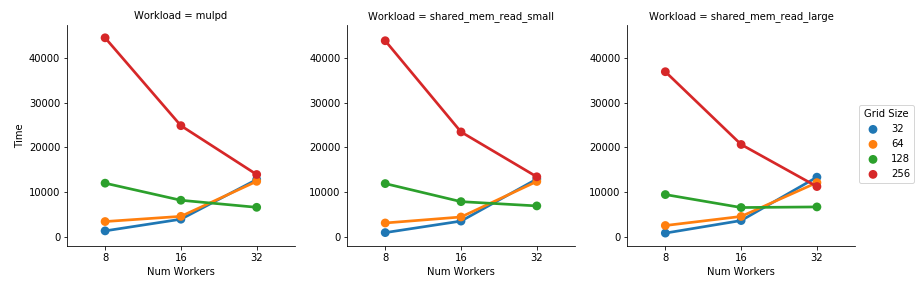
\includegraphics[width=1\textwidth]{graphics/focustest2_2.png}

\subsection{Third}

Next, we focused on the mulpd kernel, and and tested a variety of kernel repeats, and smoe more fine grained grid sizes. This is so that we could identify the point at which, as the grid size shrinks, increasing the number of threads will be sub-optimal.

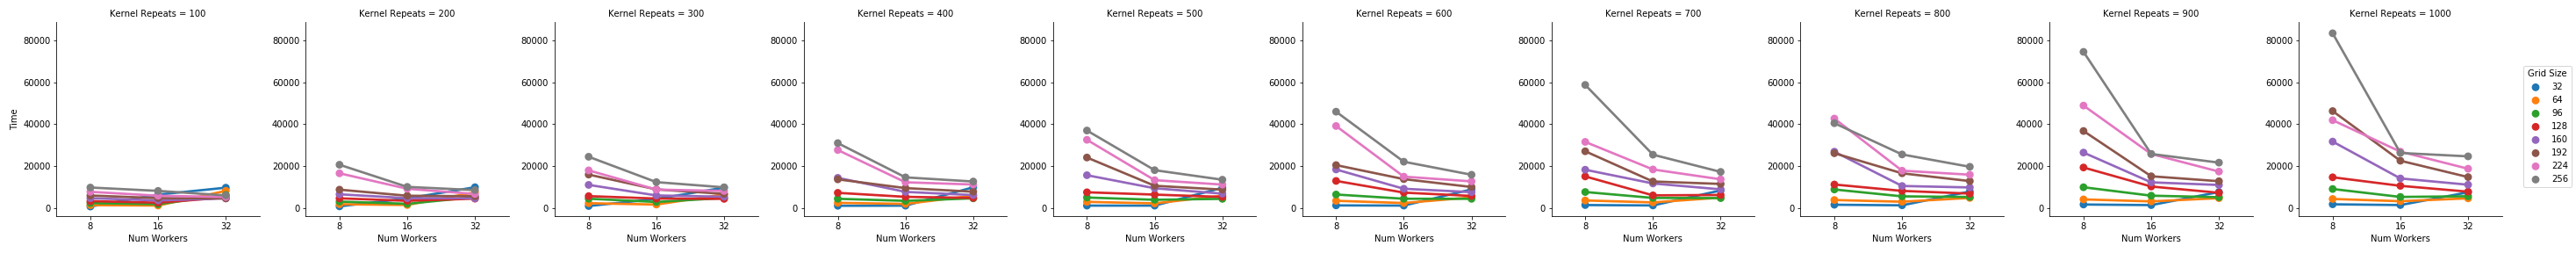
\includegraphics[width=1\textwidth]{graphics/focustest3_1.png}
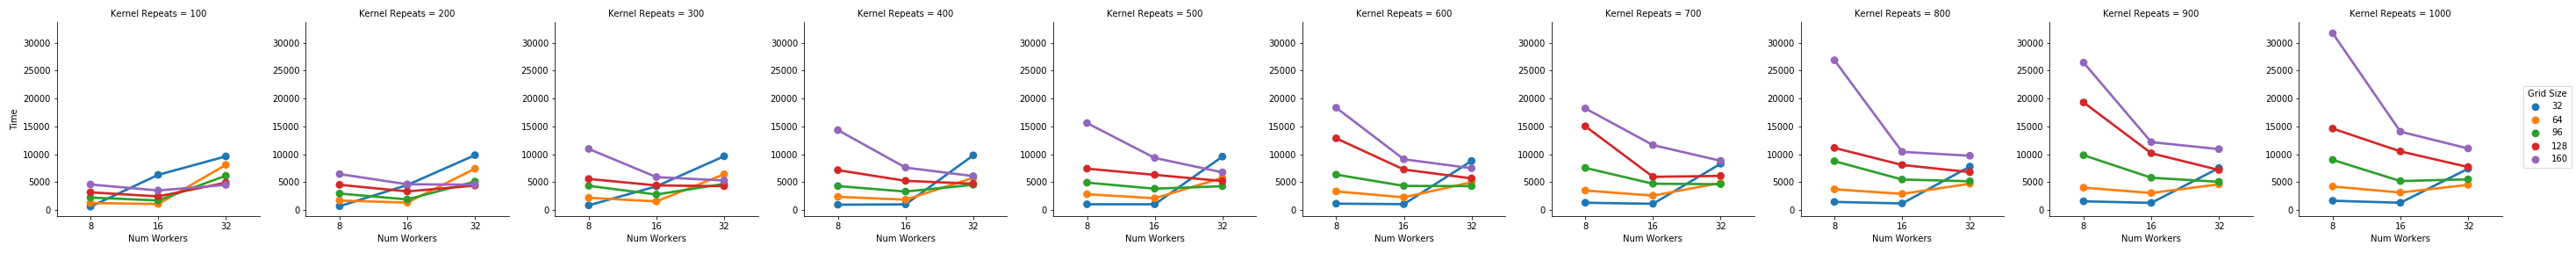
\includegraphics[width=1\textwidth]{graphics/focustest3_2.png}

As you can see from the graphs, for gridsizes 32-128, going beyond 16 threads did not increase performance in all cases.

Another interesting take from the graphs is that we can see that as the grid size increases, the runtime curves 'flip' at 32 threads such that smaller grid sizes take longer. However, as the number of kernel repeats increases, this flipping gradually lessens. This is because the increased independent workload per thread starts to 

\section{Selected Use Cases}